\documentclass{article}
\usepackage[utf8]{inputenc}
\usepackage{listings}
\usepackage{CJKutf8}
\usepackage{amsmath}
\usepackage{amssymb}
\usepackage{graphicx}
\usepackage{algorithm}
\usepackage{algpseudocode}
\usepackage{float}
\usepackage{tikz}
\usepackage{url}
\usetikzlibrary{trees}
\usepackage{subcaption}

\title{DSA HW3}
\author{B09901142 EE3 呂睿超}
\date{May 2023}

\usepackage{xcolor}

\definecolor{codegreen}{rgb}{0,0.6,0}
\definecolor{codegray}{rgb}{0.5,0.5,0.5}
\definecolor{codepurple}{rgb}{0.58,0,0.82}
\definecolor{backcolour}{rgb}{0.95,0.95,0.92}

\lstdefinestyle{mystyle}{
    backgroundcolor=\color{backcolour},   
    commentstyle=\color{codegreen},
    keywordstyle=\color{magenta},
    numberstyle=\tiny\color{codegray},
    stringstyle=\color{codepurple},
    basicstyle=\ttfamily\footnotesize,
    breakatwhitespace=false,         
    breaklines=true,                 
    captionpos=b,                    
    keepspaces=true,                 
    numbers=left,                    
    numbersep=5pt,                  
    showspaces=false,                
    showstringspaces=false,
    showtabs=false,                  
    tabsize=2
}

\lstset{style=mystyle}

\begin{document}
\begin{CJK*}{UTF8}{bsmi}
\maketitle

\section{Problem 1 - Alexander loves sweet dumplings}
\textbf{All problems in this section are done all by myself}

\begin{enumerate}
    \item \begin{enumerate}
        \item The most efficient way to construct such string is to maximally overlapped each substring.
        \item Therefore, we can observe the prefix function and discover that we should focus on certain maximum of it.
        \item We should overlap each substring until we reach the first maximum value of the prefix function counting from the last index.
        \item For example if s = ABCAB, its prefix function would be $\pi[q] = [0,0,0,1,2]$, then we could construct t as ABCAB\textbf{CAB}....\textbf{CAB}
    \end{enumerate}
    \item \begin{enumerate}
        \item Assume there won't be collisions(spurious hit) 
        \item Calculate each representations of all substrings. Specifically, transform s[-2:-1],s[-3:-1],...,s[1:-1] into a number using the modular version of preprocessing of Rabin-Karp algorithm. Store the results into an array names as C.
        \item For each query, calculate (C[$l_1] - C[r_1$] mod(q)) and $d^{(l_1-l_2)}*$(C[$l_2] - C[r_2$] mod(q)) and check if they are equal. 
        \item Time complexity analysis: The modification of the preprocessing of Rabin-Karp algorithm doesn't affect time complexity because it is still an one pass operation. We can obtain the next value(e.g. C[-3]) from the previous value(e.g.[C[-2]]) and (e.g. s[-3]) easily by some calculation.
        Therefore, the preprocessing is still O(n). Each query cause O(1), thus all queries are O(q). 
        Overall complexity is bounded by O(n+q).
        \item Also, if ($r_1 - l_1$) $\neq$ ($r_2 - l_2$), we can easily tell that they aren't identical strings.
        \item The $d^{(l_1-l_2)}$ is to shift the substring on the right to fit the order as the substring on the left in order to have a fair comparison. $d^{(l_1-l_2)}$ term can be obtained in O(m).
    \end{enumerate}
    \item \begin{enumerate}
        \item We can utilize the prefix function to find the answer.
        \item First, check the last value of the prefix function i.e. $\pi[-1]$, store it as b.
        \item Next, store n-b to a.
        \item Check $\frac{b}{a}+1$, if b < a, we can conclude that there isn't any integers other than 1 that satisfies.
        \item if b>=a ,factor it to find it's number of factor.
        \item The time consuming part is to find the prefix function, which is O(n)(satisfies the question)
    \end{enumerate}    
    \item \begin{enumerate}
        \item The modified prefix function is constructed as the following definition.
        \item Instead of finding the longest suffix that is also the prefix, we define the prefix function as finding the longest suffix substring that has a smaller lexicographical order than the prefix substring.
        \item In the original KMP algorithm, there are three circumstances we change them to the following three circumstances \begin{enumerate}
            \item while q $>$ 0 and P[q+1] $>$ T[i] : q = $\pi[q]$
            \item if P[q+1] == T[i] : q = q+1
            \item if P[q+1] $<$ T[i] : print "Pattern occurs with shift "i-m",break
            
        \end{enumerate}
    \end{enumerate}
    \item 
    \begin{enumerate}
        \item An counterexample that will produce the incorrect result from the algorithm is s = 'fcbabc', key = 'fcb'.
        \item After the algorithm check both 'b's from each string, idx\_s and idx\_key would be 3.
        \item Next, the algorithm will break the inner while loop because idx\_key == 3 == m. 
        \item Therefore, when the algorithm processes 'a' and 'f' with idx\_s = 3, and idx\_key = 0, the algorithm will return idx\_ans = 3 rather than the real answer 1.
    \end{enumerate}

\end{enumerate}

\section{Problem 2 - Sorting in Linear Time}
\textbf{All problems in this section are done all by myself}
\begin{enumerate}
    \item Step 1 : [310,601,152,234,57,8]
          Step 2 : [601,8,310,234,152,57]
          Step 3 : [8,57,152,234,310,601]

    \item  
    \begin{enumerate}
        \item Algorithm as below
        \begin{algorithm}[H]
        \caption{Count\_Rev\_by\_Magic\_Counter(arr,C)}
        \begin{algorithmic}
        \State Create an array D with length n
        \For{i = 1 to n(arr.length)}
            \State insert(arr[i])
            \State Store sum(arr[i]) to D[i]
        \EndFor
        \State ans = 0
        \For{i = 1 to n(arr.length})
            \State ans += (sum(arr[i]) - 1 - D[i])
        \EndFor
        \State \Return ans
        \end{algorithmic}
        \end{algorithm}
        \item Brief introduction of my algorithm : First, I traverse through the array to insert the values in the counter. Then, observe that find reversions is equivalent to finding values that are smaller and also on the right. Therefore, sum(R) returns all values that are smaller than itself.Then, minus itself and all the values that are smaller and also on the left, which is D[i].
        \item Time complexity analysis : I do 3*n times of the two given operation, thus we can conclude that the time complexity of the algorithm is 3*N*log(K) which is bounded with O(Nlog(K))
    \end{enumerate}
 
        
    \item  \begin{enumerate}
        \item Traverse through the string and store the index of each occurrence of $\sigma$ to another array D
        \item Go through each value in D and set D[i+1] - D[i] as tmp, add $1+2+...+tmp = \frac{tmp(tmp+1)}{2}$ to ans.
        \item Brief introduction of my algorithm : First, I store where each $\sigma$ appears in the string in order to separate the string into regions that don't contain $\sigma$. Then, calculate the length of each region and easily count how many substrings it contains by $\frac{tmp(tmp+1)}{2}$
        \item Time complexity : the first traverse is O(N) because it's a one-pass traverse. The second part is also O(N) because the length of D is also bounded by O(N).
    \end{enumerate}

    
    \item \begin{enumerate}
        \item The basic idea is similar to the previous problem, but now we create an array tmp\_arr instead of only a variable tmp to store the index of the previous occurrence of certain character.
        \item First, initialize the tmp\_arr with all 0's (length C),initialize ans = 0.
        \item Traverse the string, for each character do the following steps 
        \item Match each character to set C (assume the hash value is h).
        \item  ans+= current index $\frac{(i- tmp\_arr[h]) (i- tmp\_arr[h]+1)}{2}$ (Note: temp\_arr[h]the previous index stored in tmp\_arr) 
        \item Store the current index i to the tmp\_arr[h], and continue traversing.
        \item Time complexity : the initialize of tmp\_arr costs O(C), the one pass traversing costs O(N). Therefore, overall complexity is O(N+C).
    \end{enumerate} 
     
    
\end{enumerate}

\section{Problem 3 - Fans of H7Lin}
\textbf{All problems in this section are done all by myself}
\begin{enumerate}
    \item \begin{enumerate}
        \item  The testcase and program output are as the following screenshots. 
        \begin{figure}[H]
        \centering
    \begin{subfigure}{.5\textwidth}
      \centering
      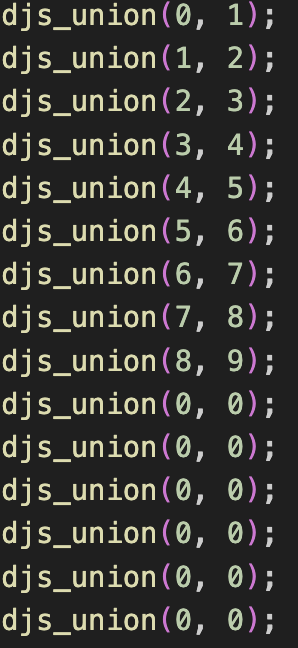
\includegraphics[width=.3\linewidth]{1testcase.png}
      \caption{Testcase}
      \label{fig:sub1}
    \end{subfigure}%
    \begin{subfigure}{.5\textwidth}
      \centering
      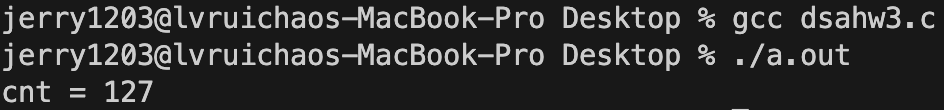
\includegraphics[width=1.2\linewidth]{1result.png}
      \caption{Program output}
      \label{fig:sub2}
    \end{subfigure}
    \caption{Figures for Problem 3-1}
    \label{fig:test}
    \end{figure}
    
    \item I checked the traversing path of each step and discover that under this random seed, find-set(0) would traverse a long distance to find the leader 9. (Based on the previous 9 unions)
    \item Therefore, for this problem I just repeatedly call Union(0,0) to trigger find-set(0) many times.
    \end{enumerate}
    \item\begin{enumerate}
        \item  The testcase and program output are as the following screenshots. 
        \begin{figure}[H]
        \centering
    \begin{subfigure}{.5\textwidth}
      \centering
      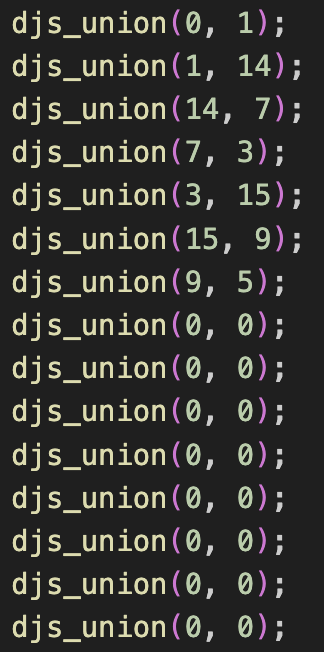
\includegraphics[width=.3\linewidth]{testcase.png}
      \caption{Testcase}
      \label{fig:sub1}
    \end{subfigure}%
    \begin{subfigure}{.5\textwidth}
      \centering
      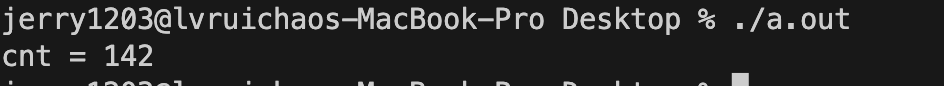
\includegraphics[width=1.2\linewidth]{result.png}
      \caption{Program output}
      \label{fig:sub2}
    \end{subfigure}
    \caption{Figures for Problem 3-2}
    \label{fig:test}
    \end{figure}
    
    \item I checked the random number in the ind array to check the relationships of each rank. Next, I union the sets following the sequence of the smallest rank to the largest.
    \item Thus when I call Union(0,0), the Find-set(0) will traverse the path one by one to the largest rank which is the leader. This path is the longest path that can be constructed, it is similar to doing search to a skewed BST.
    \end{enumerate}    
    \item \begin{enumerate}
        \item Preprocessing : make n+m sets for each row and column. MAKE-SET($r_i$ or $c_i$)
        \item INSTALL(x,y,flag) : \begin{enumerate}
            \item if flag = 0 : Union($r_x$,$r_y$)
            \item if flag = 1 : Union($c_x$,$c_y$)
        \end{enumerate} 
        \item QUERY(x,y) : Check if FIND-SET($r_0$) == FIND-SET($r_x$) and FIND-SET($c_0$) == FIND-SET($c_y$)
        \item Time complexity analysis : Follow the hint in the question \textit{From the textbook, we know that a sequence of M MAKE-SET(x), FIND-SET(x), and UNION(x,y) operations, N of which are MAKE-SET(x), can be performed in worst-case time O(Mα(N))}, in this implementation we do at most n+m MAKE-SET operations, Q FIND-SET or UNION operations , resulting in overall complexity O((n+m+Q)α(n+m)).
    \end{enumerate}

    \item 
    

    \item \begin{enumerate}
        \item Sort all the pair ($l_i,r_i$) by the value of $l_i$, and store the sequence of the Q INSTALL operations in this order.
        \item Create an empty array r\_s to store the $r_i$ of the incoming installing events.
        item Preprocessing : make n+m sets for each row and column. MAKE-SET($row_i$ or $c_i$) (in this problem I use $row_i$ instead of $r_i$ to avoid similarities)
        \item INSTALL\_v3(x,y,flag,$l_i$,$r_i$) : \begin{enumerate}
            \item if flag = 0 : Union($row_x$,$row_y$), store $r_i$ to r\_s
            \item if flag = 1 : Union($c_x$,$c_y$), store $r_i$ to r\_s
        \end{enumerate} 
        \item QUERY(x,y,t) : \begin{enumerate}
            \item Check the $l_i$ of the incoming installing event. If $l_i$  = t, do    INSTALL\_v3(x,y,flag,$l_i$,$r_i$)
            \item Check the r\_s array from the backward, if the currently checking $r_i$ < t, UNDO().
            Repeatedly traverse until the currently checking $r_i$ $\geq$ t, break.
            \item Check if FIND-SET($row_0$) == FIND-SET($row_x$) and FIND-SET($c_0$) == FIND-SET($c_y$)
         \end{enumerate}
         \item Time complexity analysis : n+m MAKE-SET costs O(n+m), Q INSTALL costs O(Q(log(n+m)), T QUERIES costs O((T+2Q)log(n+m)). Therefore, overall time complexity is O(n+m+(T+Q)log(n+m))
    \end{enumerate}
    
\end{enumerate}

\end{CJK*}
\end{document}
